
%% bare_jrnl.tex
%% V1.4b
%% 2015/08/26
%% by Michael Shell
%% see http://www.michaelshell.org/
%% for current contact information.
%%
%% This is a skeleton file demonstrating the use of IEEEtran.cls
%% (requires IEEEtran.cls version 1.8b or later) with an IEEE
%% journal paper.
%%
%% Support sites:
%% http://www.michaelshell.org/tex/ieeetran/
%% http://www.ctan.org/pkg/ieeetran
%% and
%% http://www.ieee.org/

%%*************************************************************************
%% Legal Notice:
%% This code is offered as-is without any warranty either expressed or
%% implied; without even the implied warranty of MERCHANTABILITY or
%% FITNESS FOR A PARTICULAR PURPOSE! 
%% User assumes all risk.
%% In no event shall the IEEE or any contributor to this code be liable for
%% any damages or losses, including, but not limited to, incidental,
%% consequential, or any other damages, resulting from the use or misuse
%% of any information contained here.
%%
%% All comments are the opinions of their respective authors and are not
%% necessarily endorsed by the IEEE.
%%
%% This work is distributed under the LaTeX Project Public License (LPPL)
%% ( http://www.latex-project.org/ ) version 1.3, and may be freely used,
%% distributed and modified. A copy of the LPPL, version 1.3, is included
%% in the base LaTeX documentation of all distributions of LaTeX released
%% 2003/12/01 or later.
%% Retain all contribution notices and credits.
%% ** Modified files should be clearly indicated as such, including  **
%% ** renaming them and changing author support contact information. **
%%*************************************************************************


% *** Authors should verify (and, if needed, correct) their LaTeX system  ***
% *** with the testflow diagnostic prior to trusting their LaTeX platform ***
% *** with production work. The IEEE's font choices and paper sizes can   ***
% *** trigger bugs that do not appear when using other class files.       ***                          ***
% The testflow support page is at:
% http://www.michaelshell.org/tex/testflow/



\documentclass[journal]{IEEEtran}
%
% If IEEEtran.cls has not been installed into the LaTeX system files,
% manually specify the path to it like:
% \documentclass[journal]{../sty/IEEEtran}





% Some very useful LaTeX packages include:
% (uncomment the ones you want to load)


% *** MISC UTILITY PACKAGES ***
%
%\usepackage{ifpdf}
% Heiko Oberdiek's ifpdf.sty is very useful if you need conditional
% compilation based on whether the output is pdf or dvi.
% usage:
% \ifpdf
%   % pdf code
% \else
%   % dvi code
% \fi
% The latest version of ifpdf.sty can be obtained from:
% http://www.ctan.org/pkg/ifpdf
% Also, note that IEEEtran.cls V1.7 and later provides a builtin
% \ifCLASSINFOpdf conditional that works the same way.
% When switching from latex to pdflatex and vice-versa, the compiler may
% have to be run twice to clear warning/error messages.






% *** CITATION PACKAGES ***
%
%\usepackage{cite}
% cite.sty was written by Donald Arseneau
% V1.6 and later of IEEEtran pre-defines the format of the cite.sty package
% \cite{} output to follow that of the IEEE. Loading the cite package will
% result in citation numbers being automatically sorted and properly
% "compressed/ranged". e.g., [1], [9], [2], [7], [5], [6] without using
% cite.sty will become [1], [2], [5]--[7], [9] using cite.sty. cite.sty's
% \cite will automatically add leading space, if needed. Use cite.sty's
% noadjust option (cite.sty V3.8 and later) if you want to turn this off
% such as if a citation ever needs to be enclosed in parenthesis.
% cite.sty is already installed on most LaTeX systems. Be sure and use
% version 5.0 (2009-03-20) and later if using hyperref.sty.
% The latest version can be obtained at:
% http://www.ctan.org/pkg/cite
% The documentation is contained in the cite.sty file itself.






% *** GRAPHICS RELATED PACKAGES ***
%
\ifCLASSINFOpdf
  % \usepackage[pdftex]{graphicx}
  % declare the path(s) where your graphic files are
  % \graphicspath{{../pdf/}{../jpeg/}}
  % and their extensions so you won't have to specify these with
  % every instance of \includegraphics
  % \DeclareGraphicsExtensions{.pdf,.jpeg,.png}
\else
  % or other class option (dvipsone, dvipdf, if not using dvips). graphicx
  % will default to the driver specified in the system graphics.cfg if no
  % driver is specified.
  % \usepackage[dvips]{graphicx}
  % declare the path(s) where your graphic files are
  % \graphicspath{{../eps/}}
  % and their extensions so you won't have to specify these with
  % every instance of \includegraphics
  % \DeclareGraphicsExtensions{.eps}
\fi
% graphicx was written by David Carlisle and Sebastian Rahtz. It is
% required if you want graphics, photos, etc. graphicx.sty is already
% installed on most LaTeX systems. The latest version and documentation
% can be obtained at: 
% http://www.ctan.org/pkg/graphicx
% Another good source of documentation is "Using Imported Graphics in
% LaTeX2e" by Keith Reckdahl which can be found at:
% http://www.ctan.org/pkg/epslatex
%
% latex, and pdflatex in dvi mode, support graphics in encapsulated
% postscript (.eps) format. pdflatex in pdf mode supports graphics
% in .pdf, .jpeg, .png and .mps (metapost) formats. Users should ensure
% that all non-photo figures use a vector format (.eps, .pdf, .mps) and
% not a bitmapped formats (.jpeg, .png). The IEEE frowns on bitmapped formats
% which can result in "jaggedy"/blurry rendering of lines and letters as
% well as large increases in file sizes.
%
% You can find documentation about the pdfTeX application at:
% http://www.tug.org/applications/pdftex





% *** MATH PACKAGES ***
%
%\usepackage{amsmath}
% A popular package from the American Mathematical Society that provides
% many useful and powerful commands for dealing with mathematics.
%
% Note that the amsmath package sets \interdisplaylinepenalty to 10000
% thus preventing page breaks from occurring within multiline equations. Use:
%\interdisplaylinepenalty=2500
% after loading amsmath to restore such page breaks as IEEEtran.cls normally
% does. amsmath.sty is already installed on most LaTeX systems. The latest
% version and documentation can be obtained at:
% http://www.ctan.org/pkg/amsmath





% *** SPECIALIZED LIST PACKAGES ***
%
%\usepackage{algorithmic}
% algorithmic.sty was written by Peter Williams and Rogerio Brito.
% This package provides an algorithmic environment fo describing algorithms.
% You can use the algorithmic environment in-text or within a figure
% environment to provide for a floating algorithm. Do NOT use the algorithm
% floating environment provided by algorithm.sty (by the same authors) or
% algorithm2e.sty (by Christophe Fiorio) as the IEEE does not use dedicated
% algorithm float types and packages that provide these will not provide
% correct IEEE style captions. The latest version and documentation of
% algorithmic.sty can be obtained at:
% http://www.ctan.org/pkg/algorithms
% Also of interest may be the (relatively newer and more customizable)
% algorithmicx.sty package by Szasz Janos:
% http://www.ctan.org/pkg/algorithmicx




% *** ALIGNMENT PACKAGES ***
%
%\usepackage{array}
% Frank Mittelbach's and David Carlisle's array.sty patches and improves
% the standard LaTeX2e array and tabular environments to provide better
% appearance and additional user controls. As the default LaTeX2e table
% generation code is lacking to the point of almost being broken with
% respect to the quality of the end results, all users are strongly
% advised to use an enhanced (at the very least that provided by array.sty)
% set of table tools. array.sty is already installed on most systems. The
% latest version and documentation can be obtained at:
% http://www.ctan.org/pkg/array


% IEEEtran contains the IEEEeqnarray family of commands that can be used to
% generate multiline equations as well as matrices, tables, etc., of high
% quality.




% *** SUBFIGURE PACKAGES ***
%\ifCLASSOPTIONcompsoc
%  \usepackage[caption=false,font=normalsize,labelfont=sf,textfont=sf]{subfig}
%\else
%  \usepackage[caption=false,font=footnotesize]{subfig}
%\fi
% subfig.sty, written by Steven Douglas Cochran, is the modern replacement
% for subfigure.sty, the latter of which is no longer maintained and is
% incompatible with some LaTeX packages including fixltx2e. However,
% subfig.sty requires and automatically loads Axel Sommerfeldt's caption.sty
% which will override IEEEtran.cls' handling of captions and this will result
% in non-IEEE style figure/table captions. To prevent this problem, be sure
% and invoke subfig.sty's "caption=false" package option (available since
% subfig.sty version 1.3, 2005/06/28) as this is will preserve IEEEtran.cls
% handling of captions.
% Note that the Computer Society format requires a larger sans serif font
% than the serif footnote size font used in traditional IEEE formatting
% and thus the need to invoke different subfig.sty package options depending
% on whether compsoc mode has been enabled.
%
% The latest version and documentation of subfig.sty can be obtained at:
% http://www.ctan.org/pkg/subfig




% *** FLOAT PACKAGES ***
%
%\usepackage{fixltx2e}
% fixltx2e, the successor to the earlier fix2col.sty, was written by
% Frank Mittelbach and David Carlisle. This package corrects a few problems
% in the LaTeX2e kernel, the most notable of which is that in current
% LaTeX2e releases, the ordering of single and double column floats is not
% guaranteed to be preserved. Thus, an unpatched LaTeX2e can allow a
% single column figure to be placed prior to an earlier double column
% figure.
% Be aware that LaTeX2e kernels dated 2015 and later have fixltx2e.sty's
% corrections already built into the system in which case a warning will
% be issued if an attempt is made to load fixltx2e.sty as it is no longer
% needed.
% The latest version and documentation can be found at:
% http://www.ctan.org/pkg/fixltx2e


%\usepackage{stfloats}
% stfloats.sty was written by Sigitas Tolusis. This package gives LaTeX2e
% the ability to do double column floats at the bottom of the page as well
% as the top. (e.g., "\begin{figure*}[!b]" is not normally possible in
% LaTeX2e). It also provides a command:
%\fnbelowfloat
% to enable the placement of footnotes below bottom floats (the standard
% LaTeX2e kernel puts them above bottom floats). This is an invasive package
% which rewrites many portions of the LaTeX2e float routines. It may not work
% with other packages that modify the LaTeX2e float routines. The latest
% version and documentation can be obtained at:
% http://www.ctan.org/pkg/stfloats
% Do not use the stfloats baselinefloat ability as the IEEE does not allow
% \baselineskip to stretch. Authors submitting work to the IEEE should note
% that the IEEE rarely uses double column equations and that authors should try
% to avoid such use. Do not be tempted to use the cuted.sty or midfloat.sty
% packages (also by Sigitas Tolusis) as the IEEE does not format its papers in
% such ways.
% Do not attempt to use stfloats with fixltx2e as they are incompatible.
% Instead, use Morten Hogholm'a dblfloatfix which combines the features
% of both fixltx2e and stfloats:
%
% \usepackage{dblfloatfix}
% The latest version can be found at:
% http://www.ctan.org/pkg/dblfloatfix




%\ifCLASSOPTIONcaptionsoff
%  \usepackage[nomarkers]{endfloat}
% \let\MYoriglatexcaption\caption
% \renewcommand{\caption}[2][\relax]{\MYoriglatexcaption[#2]{#2}}
%\fi
% endfloat.sty was written by James Darrell McCauley, Jeff Goldberg and 
% Axel Sommerfeldt. This package may be useful when used in conjunction with 
% IEEEtran.cls'  captionsoff option. Some IEEE journals/societies require that
% submissions have lists of figures/tables at the end of the paper and that
% figures/tables without any captions are placed on a page by themselves at
% the end of the document. If needed, the draftcls IEEEtran class option or
% \CLASSINPUTbaselinestretch interface can be used to increase the line
% spacing as well. Be sure and use the nomarkers option of endfloat to
% prevent endfloat from "marking" where the figures would have been placed
% in the text. The two hack lines of code above are a slight modification of
% that suggested by in the endfloat docs (section 8.4.1) to ensure that
% the full captions always appear in the list of figures/tables - even if
% the user used the short optional argument of \caption[]{}.
% IEEE papers do not typically make use of \caption[]'s optional argument,
% so this should not be an issue. A similar trick can be used to disable
% captions of packages such as subfig.sty that lack options to turn off
% the subcaptions:
% For subfig.sty:
% \let\MYorigsubfloat\subfloat
% \renewcommand{\subfloat}[2][\relax]{\MYorigsubfloat[]{#2}}
% However, the above trick will not work if both optional arguments of
% the \subfloat command are used. Furthermore, there needs to be a
% description of each subfigure *somewhere* and endfloat does not add
% subfigure captions to its list of figures. Thus, the best approach is to
% avoid the use of subfigure captions (many IEEE journals avoid them anyway)
% and instead reference/explain all the subfigures within the main caption.
% The latest version of endfloat.sty and its documentation can obtained at:
% http://www.ctan.org/pkg/endfloat
%
% The IEEEtran \ifCLASSOPTIONcaptionsoff conditional can also be used
% later in the document, say, to conditionally put the References on a 
% page by themselves.




% *** PDF, URL AND HYPERLINK PACKAGES ***
%
%\usepackage{url}
% url.sty was written by Donald Arseneau. It provides better support for
% handling and breaking URLs. url.sty is already installed on most LaTeX
% systems. The latest version and documentation can be obtained at:
% http://www.ctan.org/pkg/url
% Basically, \url{my_url_here}.




% *** Do not adjust lengths that control margins, column widths, etc. ***
% *** Do not use packages that alter fonts (such as pslatex).         ***
% There should be no need to do such things with IEEEtran.cls V1.6 and later.
% (Unless specifically asked to do so by the journal or conference you plan
% to submit to, of course. )


% correct bad hyphenation here
\hyphenation{op-tical net-works semi-conduc-tor}

% custom includes
\usepackage{cite}
\usepackage{amsmath, amssymb}
\usepackage{float}
\usepackage{graphicx}
\usepackage{subcaption}

\DeclareMathOperator*{\argmax}{arg\,max}

\begin{document}
%
% paper title
% Titles are generally capitalized except for words such as a, an, and, as,
% at, but, by, for, in, nor, of, on, or, the, to and up, which are usually
% not capitalized unless they are the first or last word of the title.
% Linebreaks \\ can be used within to get better formatting as desired.
% Do not put math or special symbols in the title.
\title{Computational RNA Structure Prediction}
%
%
% author names and IEEE memberships
% note positions of commas and nonbreaking spaces ( ~ ) LaTeX will not break
% a structure at a ~ so this keeps an author's name from being broken across
% two lines.
% use \thanks{} to gain access to the first footnote area
% a separate \thanks must be used for each paragraph as LaTeX2e's \thanks
% was not built to handle multiple paragraphs
%

\author{Samuel~Jackson,~University~Of~Aberystwyth}

% note the % following the last \IEEEmembership and also \thanks - 
% these prevent an unwanted space from occurring between the last author name
% and the end of the author line. i.e., if you had this:
% 
% \author{....lastname \thanks{...} \thanks{...} }
%                     ^------------^------------^----Do not want these spaces!
%
% a space would be appended to the last name and could cause every name on that
% line to be shifted left slightly. This is one of those "LaTeX things". For
% instance, "\textbf{A} \textbf{B}" will typeset as "A B" not "AB". To get
% "AB" then you have to do: "\textbf{A}\textbf{B}"
% \thanks is no different in this regard, so shield the last } of each \thanks
% that ends a line with a % and do not let a space in before the next \thanks.
% Spaces after \IEEEmembership other than the last one are OK (and needed) as
% you are supposed to have spaces between the names. For what it is worth,
% this is a minor point as most people would not even notice if the said evil
% space somehow managed to creep in.



% The paper headers
%\markboth{Journal of \LaTeX\ Class Files,~Vol.~14, No.~8, August~2015}%
%{Shell \MakeLowercase{\textit{et al.}}: Bare Demo of IEEEtran.cls for IEEE Journals}
% The only time the second header will appear is for the odd numbered pages
% after the title page when using the twoside option.
% 
% *** Note that you probably will NOT want to include the author's ***
% *** name in the headers of peer review papers.                   ***
% You can use \ifCLASSOPTIONpeerreview for conditional compilation here if
% you desire.




% If you want to put a publisher's ID mark on the page you can do it like
% this:
%\IEEEpubid{0000--0000/00\$00.00~\copyright~2015 IEEE}
% Remember, if you use this you must call \IEEEpubidadjcol in the second
% column for its text to clear the IEEEpubid mark.



% use for special paper notices
%\IEEEspecialpapernotice{(Invited Paper)}




% make the title area
\maketitle

% As a general rule, do not put math, special symbols or citations
% in the abstract or keywords.
\begin{abstract}
The abstract goes here.
\end{abstract}

% Note that keywords are not normally used for peerreview papers.
\begin{IEEEkeywords}
RNA, literature review, dynamic programming, context free grammars, bioinformatics, computational biology.
\end{IEEEkeywords}






% For peer review papers, you can put extra information on the cover
% page as needed:
% \ifCLASSOPTIONpeerreview
% \begin{center} \bfseries EDICS Category: 3-BBND \end{center}
% \fi
%
% For peerreview papers, this IEEEtran command inserts a page break and
% creates the second title. It will be ignored for other modes.
\IEEEpeerreviewmaketitle



\section{Introduction}
\label{sec:intro}

Ribonucleic acid (RNA) is diverse set of fundamental biological macromolecules that play an important part in many biological processes. An understanding of the structure of different types of RNA molecules can further our understanding of the molecular machinery at work inside our body as well as have direct practical applications to modern medicine by controlling protein synthesis, transcription, and virus replication \cite{schlick2010molecular}.

The primary structure of bases in a strand of RNA is fairly easy to obtain experimentally through rapid sequencing methods. Experimental determination of RNA secondary and tertiary RNA structure to an atomistic level of resolution is typically performed using either by X-ray crystallography or NMR spectroscopy. However secondary and tertiary structure determination has a bottleneck due to the diverseness of RNA molecules and the cost of experimental determination methods\cite{ya2014rna}. This leaves a high number of RNA with determined primary structure but little or no information about their the secondary or tertiary structure.

RNA structure prediction is the field of bioinformatics which aims to accurately predict the secondary and tertiary structure of RNA from the known primary structure. This is a difficult procedure due to the non-trivial structures that can be formed by as an RNA molecule folds and binds with itself. Another limitation is the high number of potentially feasible but sub-optimum structures that inhabit the conformational space close to the true structure. Structure prediction also suffers from a ``catch-22'' scenario where the quality of predictions could potentially be made better if only more known structures could be determined. Most approaches, both for secondary and tertiary structure focus are based on predicting the structure which exhibits the minimum of free energy of the chemical structure, but this is still an imperfect simplification.

This paper provides a review many of the methods used to predict both the secondary and tertiary structure of RNA molecules. Section \ref{sec:rna-structure} provides an overview of the chemical structure of RNA from the basic building blocks up to the full 3D structure. Section \ref{sec:rna-secondary-structure} discusses various methods applied to predicting the secondary structure of RNA. Section \ref{sec:rna-tertiary-structure} provides the complementary discussion on the prediction of the tertiary structure of RNA. A summary and discussion of the challenges faced and overcome in both types of structure prediction is provided in section \ref{sec:discussion}. Finally, some concluding remarks as well as some comments of future directions are given in section \ref{sec:conclusion}.


\section{RNA Structure}
\label{sec:rna-structure}
RNA molecules come in a wide variety of different shapes, sizes, and functions. One of the most important types of RNA is messenger RNA (mRNA) which is responsible for carrying information about the amino acid sequence required to build a protein from DNA strands in the cell nucleus to the ribosome for protein synthesis. However, many types of RNA are non-coding, i.e. they do not play a direct part carrying the coding information for protein translation. Instead they for part of the complex system of cellular machinery. An example of non-coding RNA is ribosomal RNA (rRNA) which act as the catalysts in the ribosome for protein synthesis. Transfer RNA (tRNA) are yet another part of the translation process which delivers an amino acid to the ribosome according to a codon of mRNA. RNAs can also act in a regulatory role by down-regulating gene expression in the translation process. RNA molecules can also act as the genome for viruses, such as Ebola, HIV, and SARS which can utilise proteins to replicate themselves.

RNA is typically found as single stranded molecules in nature where parts of the of the strand is folded upon itself. This is in contrast to DNA which are typically composed of multiple strands which bond with one another. RNA folding, the process by which an RNA strand bonds with itself to form complicated 3D structures, can be classified into three different categories: primary, secondary, and tertiary structure. The remainder of this section defines the different categories of structure and what they mean in terms of RNA folding.

\subsection{Primary Structure}
\label{subsec:primary-structure}

 The primary structure refers to the sequence of building blocks of RNA. Each strand of RNA is made up of a sequence of organic chemicals called nucleotides. Nucleotides can be split into a three major components: a five carbon sugar ring (ribose), a phosphate group, and a nitrogenous base. The nitrogenous base can be one of four biological compounds: the nucleobases adenine, cytosine, guanine, and uracil, commonly abbreviated to the first letter of each molecule (A, C, G, and U). Nucleotides form the repeating units of a strand of RNA. A collection of nucleotides form a nucleic acid through a phosphodiester bond connecting the 5$'$ carbon on the ribose ring of one nucleotide to the 3$'$ carbon of the next. Typically as strand of RNA is described using the abbreviated bases from the 5$'$ carbon end of the sequence towards the 3$'$ carbon end.
 
\begin{figure}[t]
\centering
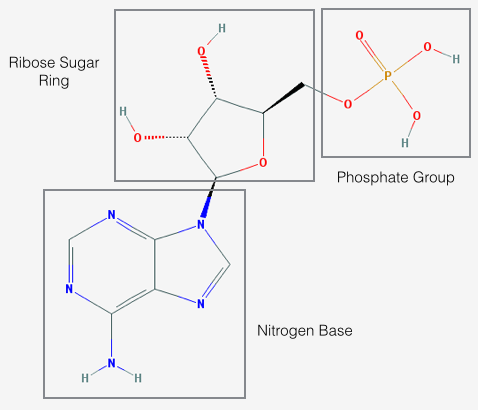
\includegraphics[width=0.5\textwidth]{img/nucleotide.png}
\caption{2D chemical structure of a nucleotide (adenosine 5$'$-monophosphate) with the adenine base (lower left), ribose sugar ring (middle) and phosphate group (upper right). 2D chemical structure source: PubChem \cite{adenine2016pubchem}.}
\label{fig:nucleotide}
\end{figure}
 
\subsection{Secondary Structure}
\label{subsec:intro-rna-sec-structure}

 Bases can be further split into two categories based on their chemical structure. Purine bases (A and G) contain a two nitrogen rings while pyrimidines (C and U) contain just a single ring. The differences in the structure of the nitrogen base allow hydrogen bonds to form between complementary pairs of nucleotides. The classic Watson-Crick base pairing scheme causes A to bond with U and C to bond with G. Other pairing schemes are possible such as Hoogsteen base pairs where the purine base is rotated and wobble base pairs where G-U base pairing is possible. The type of base pairing is important to structure prediction because different types of base pairs will have different thermodynamic stabilities associated with them which is a major factor in predicting how a molecule will fold.
 
 \begin{figure}[!tbp]
  \begin{subfigure}[b]{0.5\textwidth}
    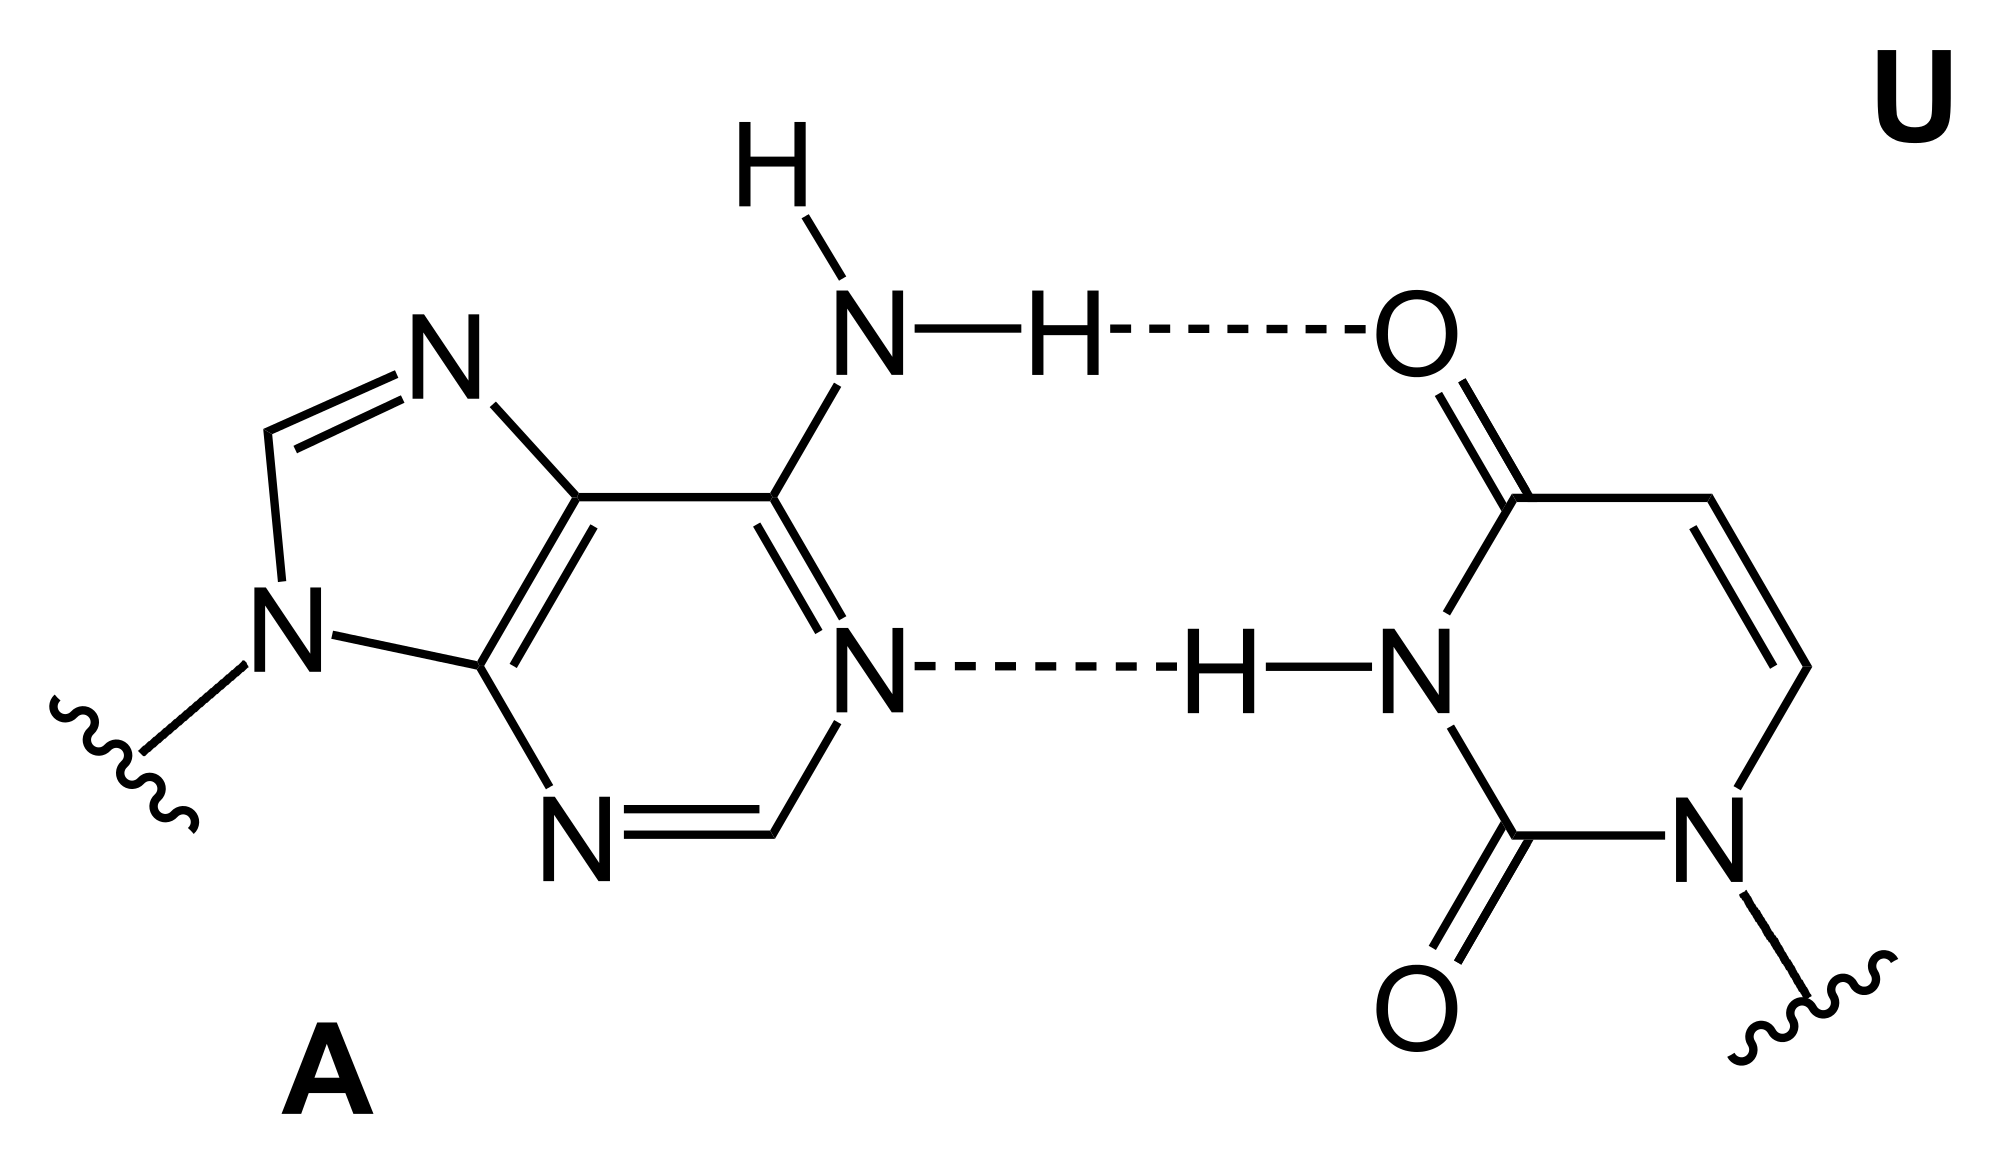
\includegraphics[width=\textwidth]{img/Base_pair_AU.png}
    \caption{Chemical structure of an adenine - uracil base pair.}
    \label{fig:au-base-pair}
  \end{subfigure}
  \hfill
  \begin{subfigure}[b]{0.5\textwidth}
    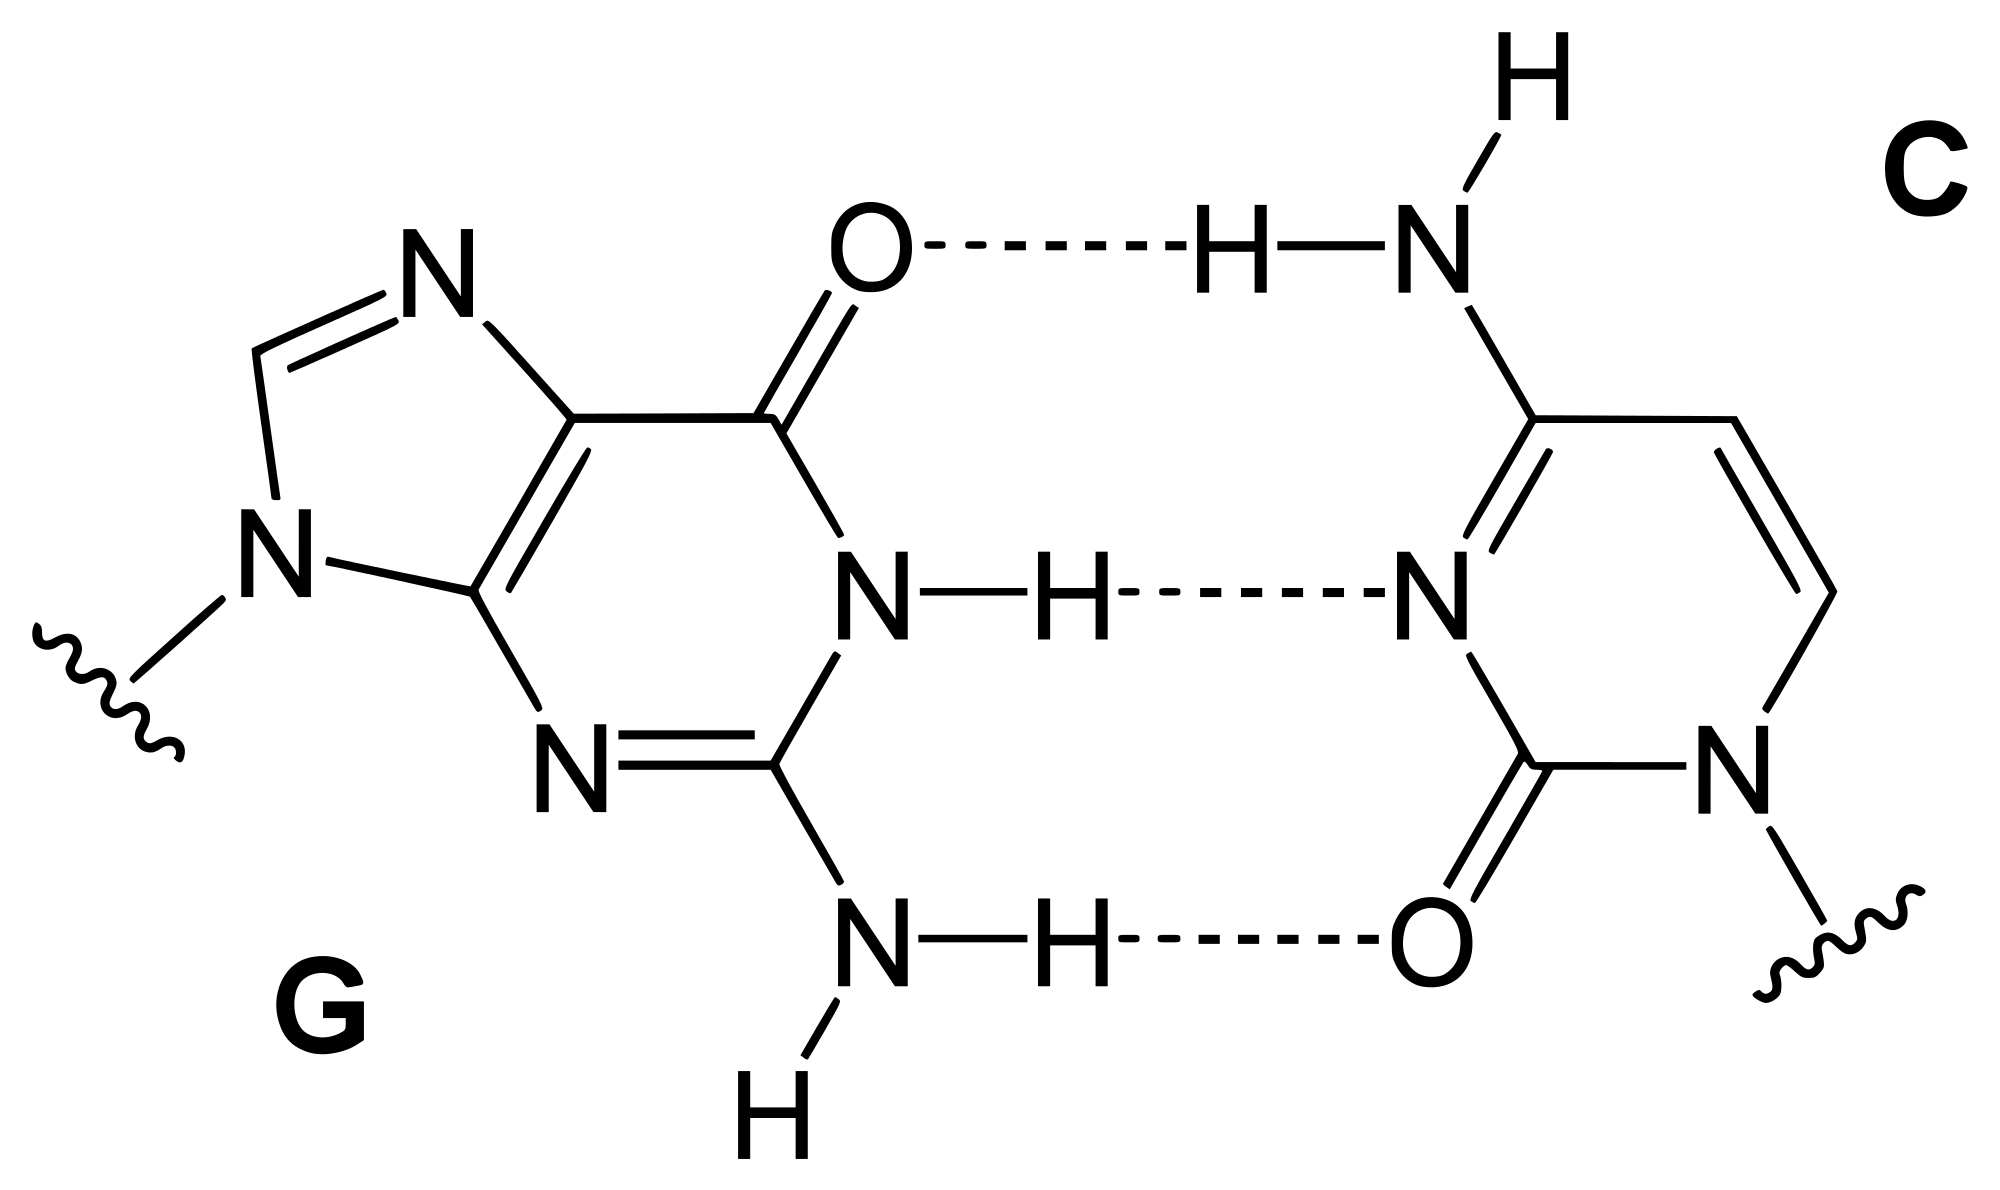
\includegraphics[width=\textwidth]{img/Base_pair_GC.png}
    \caption{Chemical structure of a guanine - cytosine base pair.}
    \label{fig:gc-base-pair}
  \end{subfigure}
  \caption{Watson-Crick base pairing in RNA. A-U and G-C form base pairs using two or three hydrogen bonds (shown as dashed lines) depending on the pair type.}
\end{figure}

The patterns of the structures that are created through base-pairing can be classified into a number of different structures. Reference \cite{nowakowski1997rna} provides a comprehensive introduction. Commonly encountered structural motifs frequently used in RNA secondary structure prediction are:

\begin{itemize}
	\item \textbf{Base pair stacks} - The most common structural element. Formed by an RNA strand folding on itself and forming hydrogen bonds between complementary bases. Bonds in base pair stacks form between two parts of the RNA each running in an anti-parallel direction to one another. 
	\item \textbf{Hairpin loops} - A collection of unpaired nucleotides at the terminus of a base pair stack. So called because the strand loops back and binds with itself.
	\item \textbf{Symmetric and asymmetric loops} - a collection of unpaired nucleotides between two base pair stacks. Symmetrical if the number of nucleotides on each side is equal, asymmetrical if not.
	\item \textbf{Bulges} - Similar to loops but with one side having no unpaired nucleotides.
	\item \textbf{Junctions} - The point at which multiple base pair stacks meet is referred to as a junction.
	\item \textbf{Pseudoknots} - Pseudoknots are formed between the unpaired nucleotides on a hairpin loop with the unpaired nucleotides on an adjacent strand. So called because the structure shows some resemblance to a mathematical knot. The properties of pseudoknots and similar structures propose a particular challenge to prediction due to the complex, interwoven, long range base pairing.
	\item \textbf{Kissing hairpins} - A variation of pseudoknots, but directly between the unpaired nucleotides of two hairpin loops.
\end{itemize}

Traditionally secondary RNA structure prediction has focussed on attempting to generate a combination of these structures based on the thermodynamic stability of the structure and the type of base pairs within the structure.

\begin{figure}[t]
\centering
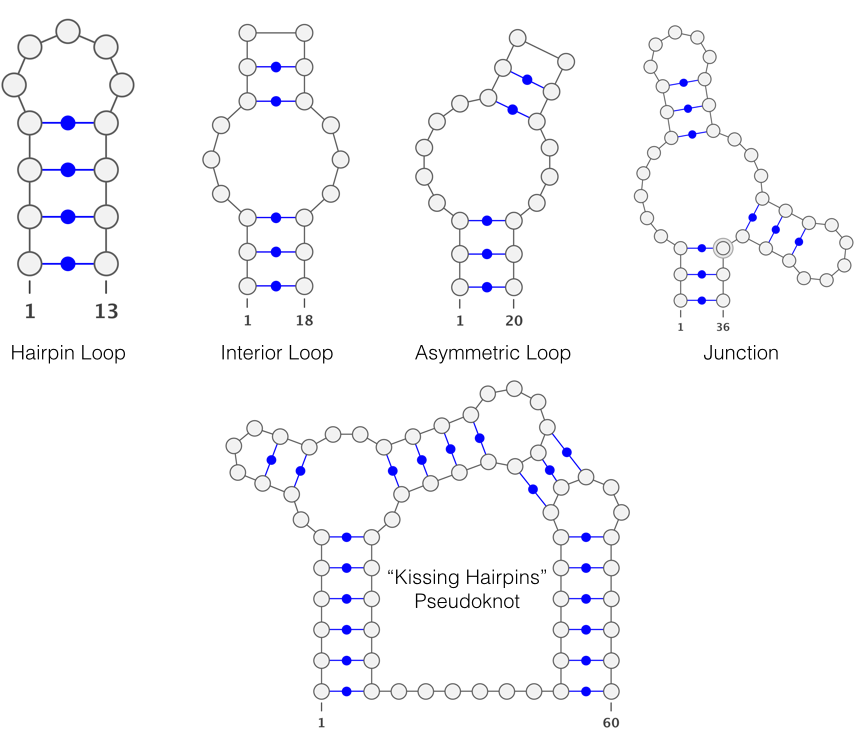
\includegraphics[width=0.5\textwidth]{img/secondary_structure_types.png}
\caption{Various types of motif present in the secondary structure of RNA molecules. The kissing hairpin pseudoknotted structure exhibits stems, hairpin loops, a junction (top left) and a pseudoknot (top right). All diagrams made with the aid of VARNA \cite{darty2009varna}.}
\label{fig:secondary-structure-types}
\end{figure}

\subsection{Tertiary Structure}
\label{subsec:intro-rna-ter-structure}
While the secondary structure of an RNA molecule can revel much about it's role, it is the tertiary structure that is the ultimate goal of structure prediction. 3D RNA folding is still very much an open problem in the bioinformatics community, but as will be revealed in the following pages much progress has already been made. The additional spatial dimension brings a wide variety of potential conformations beyond those of two dimensions.

The hydrogen bonds connecting complementary base pairs are not rigidly fixed. Individual base pairs in an RNA strand can exhibit are variety of movements (see figure \ref{fig:base-pair-interactions}). The geometry of the base pairs can be described by create a coordinate system with one axis parallel to the direction of the helical stem, one perpendicular along the direction of the bond, and one perpendicular to the bond itself:

\begin{itemize}
	\item \textbf{Stretch, Shear, and Stagger} - Each base can be translated in all axes relative to one another.

	\item \textbf{Buckle} - The dihedral rotation along the hydrogen bond causing a kink to occur in the connection between the two bases.

	\item \textbf{Propeller Twist} - The dihedral rotation about the hydrogen bond connecting a pair of bases relative to the normal of each base. The bases appear to twist like a propeller or bow-tie.
	\item \textbf{Opening} - A scissoring effect rotating the bases about the helical axis.
\end{itemize}

The bonded base pairs can also move relative together relative to the helical axis. These movements can be one of:

\begin{itemize}
	\item \textbf{X/Y Displacement} - Translation of the bonded bases in either the $x$ or $y$ directions relative to the $z$ axis.
	\item \textbf{Inclination} - Given by the angle between the long axis and the helical axis.
	\item \textbf{Tip} - The complement to inclination. This is the angle between the short axis and the helical axis. 
\end{itemize}

The geometry of two adjacent pairs of bases will also effect one another. This can be seen in the third part of diagram \ref{fig:base-pair-interactions}.

\begin{itemize}
	\item \textbf{Shift, Slide, and Rise} - Displacement between two adjacent pairs of bases along one of the three coordinate axes.
	\item \textbf{Tilt, Roll, and Twist} - Rotation about the same axes as shift, slide, and rise respectively.
\end{itemize}

Beyond the flexibility of the bonded between base pairs the rest of the nucleotide can exhibit movement in all three dimensions. The ribose sugar ring in a single nucleotide exhibits sugar puckering which introduces non-planarity to the ring structure. This can be parameterised by 5 torsion angles for the bonds between atoms in the ring typically denoted by $\tau_i$ where $i$ is the $i^{th}$ torsion angle starting from the O4$'$ to C1$'$ bond. The glycosidic bond between the ribose sugar and the base can rotate and is typically parametrised by another torsion angle labelled $\chi$. Finally, the backbone of an RNA molecule from the 5$'$ end connected to the phosphate group through the ribose sugar to the 3$'$ end of the molecule is parameterised by a set of 6 torsion angles over each bond (each shown in figure \ref{fig:backbone-torsion-angles}).

Despite the high number of parameters describing just a single nucleotide the space of potential realistic conformations is mercifully much smaller than the space of theoretical values for every parameter. For example, the values that the 6 backbone torsion angles are limited by the need to avoid steric clashes.

Beyond this parameterisation of a single nucleotide in three dimensions, folded RNA molecules also exhibit a variety of structure motifs in three dimensions. These of course include all of structure motifs present in two dimensions and described in the previous section. Higher order tertiary structural components include:

\begin{itemize}
	\item \textbf{Triplexes and Quadruplexes} - Single stranded portions of RNA can bond with a helical stack through hydrogen bonding with non-Watson-Crick pairs to form a triplex. Triplexes are a common feature in RNA, particularly at the junction between two helical stacks. Quadruplexes, where four nucleotides bond with one another, are also possible.
	\item \textbf{Coaxial stacking} - The formation of a more stable structure by the creation of a pseudoknot. This is where two single stranded regions bond with one another next to an existing stem.
	\item \textbf{Tetraloops} - Three dimensional hairpin loop structures capped with four loop nucleotides. These offer a chemically stable structure while offering a site for potential RNA-RNA or RNA-Protein interactions.
\end{itemize}

 For a more detailed discussion on the conformations of nucleotides in three dimensions the reader is directed to references \cite{neidle2010principles, schlick2010molecular, nowakowski1997rna}.

\begin{figure}[t]
\centering
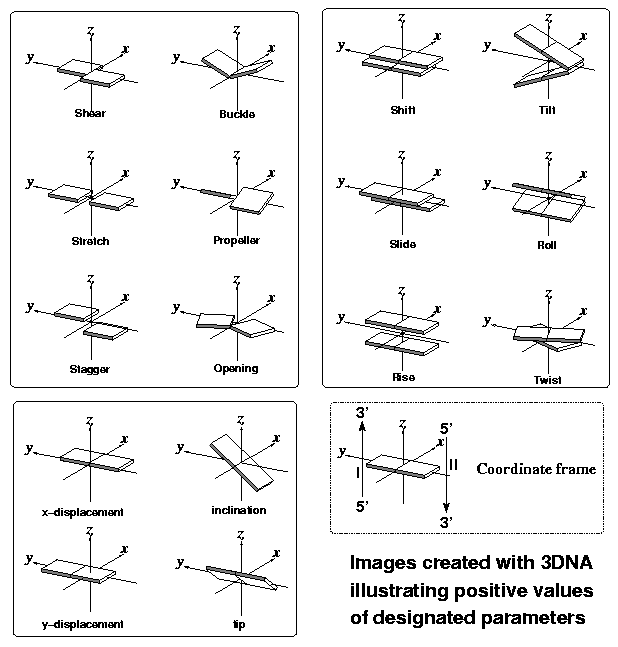
\includegraphics[width=0.5\textwidth]{img/base_pair_interactions.png}
\caption{Base pair interactions in three dimensions. Top left and bottom left: individual base pair movements relative to one another (top) and relative to the helix (bottom). Top right: possible interactions between two adjacent base pairs. Image source: Olsen et al. Copyright 2001 by Elsevier Inc. \cite{Olson2001229}.}
\label{fig:base-pair-interactions}
\end{figure}

\begin{figure}[t]
\centering
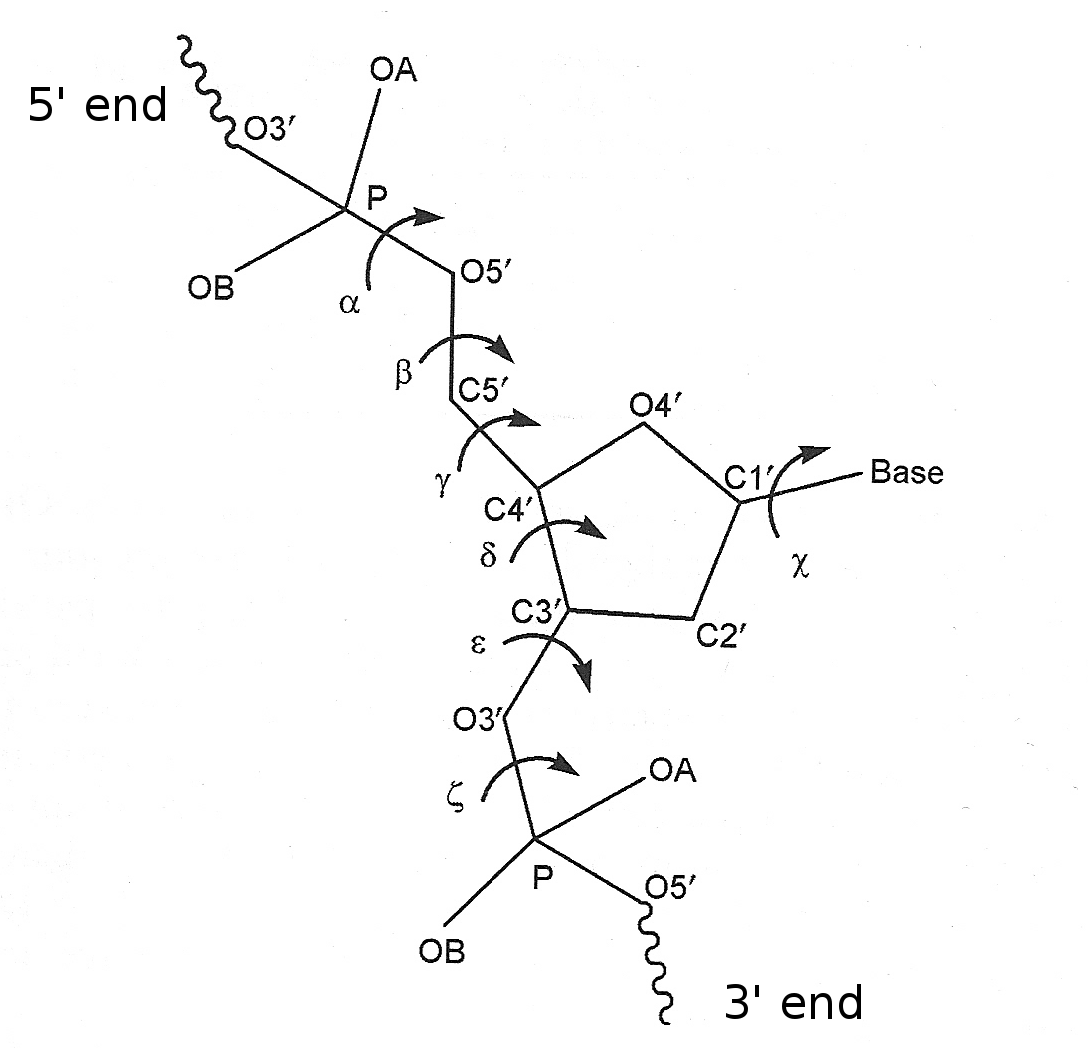
\includegraphics[width=0.5\textwidth]{img/backbone_torsion_angles.png}
\caption{Nucleic acid backbone torsion angles for a single nucleotide denoted by $\alpha$, $\beta$, $\gamma$, $\delta$, $\epsilon$, and $\zeta$. The torsion angle on glycosidic bond between the ribose sugar and base is also show as the parameter $\chi$. Image source: Stephen Neidle Copyright 2008 by Elsevier Inc. \cite{neidle2010principles}.}
\label{fig:backbone-torsion-angles}
\end{figure}

\section{RNA secondary structure prediction}
\label{sec:rna-secondary-structure}
The challenge of accurately predicting the secondary structure of RNA has a long and varied history. There are two major schools of thought in secondary structure prediction, with folding algorithms being loosely categorised as being either thermodynamic or probabilistic using stochastic context free grammar (SCFG) models. Most of the approaches to folding share deep similarities in how structure is determined. The major differences are in the scoring schemes and the parametrisation used. This section provides an overview of history prediction starting from early thermodynamic models and working forwards chronologically to more recent probabilistic models.

\begin{table*}[t]
\centering
\caption{Summary of Approaches to Secondary Structure Prediction}
\label{my-label}
\begin{tabular}{|l|l|l|l|p{5cm}|}
\hline
\textbf{Paper}                             & \textbf{Year} & \textbf{Criteria}                     & \textbf{Weighting} & \textbf{Contributions}                                                           \\ \hline
Nussinov \cite{nussinov1980fast}           & 1980          & Maximum Base Pairing                  & Binary             & Dynamic programming algorithm for base pairs                                     \\ \hline
Zuker and Stieglar \cite{zuker1981optimal} & 1981          & Minimum Free Energy                   & Thermodynamic      & Minimum free energy algorithm                                                    \\ \hline
McCaskill \cite{mccaskill1990equilibrium}  & 1990          & Partition Function Probability \& MFE & Thermodynamic      & Partition function, base pair probability matrix, melting behaviour description. \\ \hline
\end{tabular}
\end{table*}

\subsection{Thermodynamic Models}
\label{subsec:thermodynamic-models}

One of the earliest influential approaches to secondary structure prediction is the Nussinov algorithm \cite{nussinov1980fast}. The Nussinov algorithm is used to find the maximum base pairing of a sequence of nucleotides. The algorithm recursively calculates the maximum pairing for subsections of a RNA sequence. The recursive definition can be sped up using a dynamic programming table to yield an algorithm with $O(n^3)$ time and $O(n^2)$ space complexity. Little improvement on algorithmic complexity has been achieved since. 

While the Nussinov algorithm is guaranteed to produce the structure with maximum base pairs it has some major flaws. Firstly the algorithm assumes base pairs are non-crossing and cannot handle pseudo-knotted structures. Secondly, it usually does not produce biologically plausible structures. For example, the stacking orientation of base pairs and loop length are not weighted in any way. Thirdly, the algorithm only predicts a single structure. It is known that the space of possible secondary structures will often have many plausible instances close to the optimum structure \cite{mccaskill1990equilibrium}. The Nussinov algorithm provides no way of differentiating between possible sub optimum structures. 

A much more biologically feasible criteria of determining whether two bases will pair is to minimise the free energy exhibited by a structure. This is the method proposed by Zuker and Stieglar \cite{zuker1981optimal}. The underlying algorithm shares a very similar formulation as the Nussinov method but with a few key differences. Firstly their algorithm associates energy with the regions between bonds, as opposed to the bonds themselves (which is effectively what Nussinov uses). Secondly two energy functions are defined for subsequences of the string of nucleotides. These are the energy of the subsequence with and without base pairing between two given indices. Energy for the structure is recursively computed in a bottom-up fashion by taking the minimum energy at each point. The final computation should yield the secondary structure with minimum free energy (MFE).

The MFE formulation can be used to produce much more biologically plausible structures in contrast to base pair maximisation. The thermodynamic weights are used to push the algorithm away from impossible or implausible structures (such as very short hairpin loops) and towards the correct structure by giving them highly positive weights. The method also has a certain biological backing because of its basis in thermodynamics which is more realistic to how cell processes work than base pair maximisation. 

However, this method and thermodynamic based approaches in general, are limited by the accuracy of experimental studies of RNA. Many approaches rely on custom scoring rules or simply ignore aspects of reality in the model. For example, sequence dependance in RNA loop structures are often ignored due to the lack of experimental tools for assessing their free energy contribution \cite{do2006contrafold}. Many more recent prediction algorithms utilise the thermodynamic parameters used by Turner's group \cite{mathews1999expanded} as opposed to the weights used in the original paper. 

Furthermore, this still shares some of the limitations of \cite{nussinov1980fast}. The MFE algorithm cannot handle pseudo-knotted structures and can only produces a single structure rather than a distribution of likely structures. Despite these limitations thermodynamic models based on this approach are still used in abundance for secondary structure prediction and produce some of the best available results \cite{laing2010computational} \cite{rivas2013four}.

Moving forward in time, another key contribution to the area was the equilibrium partition function formulation by McCaskill \cite{mccaskill1990equilibrium}. The aim of this paper was to not only produce the MFE structure for a given sequence but to produce a visual picture of the full ensemble of alternative equilibrium structures and provides a practical method for computing probability of bases pairing. 

McCaskill describes the ensemble of RNA structures using the partition function

\begin{equation}
	Q = \sum_s e^{-(E(A)/kT)}
\end{equation} 

where $A$ is a specific structure, $E$ is the energy of a structure, $T$ is the absolute temperature in Kelvin, and $k$ is the Boltzmann constant. The probability of a specific structure $A$ given sequence $S$ is then given by

\begin{equation}
	P(A|S) = \frac{1}{Q} e^{-(E(A)/kT)}	
\end{equation}

Finally the probability of two bases $(i, j)$ pairing is given by

\begin{equation}
	P((i,j)|S) = Q_{ij} / Q
\end{equation}
where
\begin{equation}
	Q_{ij} = \sum_{(i,j) \in A} e^{-(E(A)/kT)}
\end{equation}

More complicated interactions where bases pair at hairpin loops, internal loops, and junctions are handled in further derivations excluded for brevity. McCaskill also outlines how to reduce the computational time and space complexity of the final algorithm to be $O(n^3)$ and $O(n^2)$ respectively.

Further contributions by the paper include the ``box matrix'' plot visualise the probabilities for each base pair predicted by the algorithm alongside the predicted optimal and experimental pairings. This takes the form of a matrix where each element is the probability that bases $i$ and $j$ will pair shown on a logarithmic scale in the upper left corner of the matrix. The lower right side of the matrix is then used to show the optimal pairings and optionally where the experimentally confirmed structure differs. 

The partition function formulation also encodes information about the phase transitions for the ensemble with respect to change in temperature. This provides another window into the structural properties of a RNA sequence.

Both McCaskill's partition function method and Zucker and Stieglar's MFE method remain to this day as the bedrock of many successful approaches to RNA structure prediction. Two notable extensions of these works which should be mentioned for completeness are the papers by Matthews et al. \cite{mathews1999expanded} (often referred to as the Turner group) in producing Mfold and Hofacker et al. \cite{hofacker1994fast} in producing the RNAfold and ViennaRNA packages. 

Matthews et al. improved on the set of thermodynamic parameters by extrapolating free energies obtained from analysis of representative molecules for loop structures and comparative sequence analysis for stability of tetraloops and estimate junction initiation parameters. Hofacker et al. contribute a collective package (ViennaRNA) that incorporates not only RNAfold, a parallelised MFE algorithm based on Zucker's, but also tools for inverse folding and comparison of secondary structures. 

Mfold in particular is often used as a baseline for secondary structure prediction. These methods are also often used in the calculation of secondary structure for the prediction of tertiary RNA structure \cite{laing2010computational, cruz2012rna, miao2015rna}.

A more modern free energy minimisation approach was created by Deigan et al. \cite{deigan2009accurate} which incorporates additional experimental information from SHAPE experiments into there approach. Selective 2'-hydroxyl acylation analysed by primer extension (SHAPE) experiments report differences in local nucleotide flexibility. Base pairing reduces the local flexibility associated with a nucleotide which can be related to the probability that a particular nucleotide will form a base pair. The author's propose a ``pseudo-free energy change'' term which can be added to a regular free energy model. The term has the form

\begin{equation}
	\Delta G_{SHAPE}(i) = m \cdot ln[SHAPEreactivity(i) + 1] + b
\end{equation}

where $i$ is the nucleotide number, $m$ is a parameter that penalises base pairing in nucleotides with high SHAPE reactivities and $b$ is parameter which is negative and represents an increment in free energy for nucleotides which exhibit low SHAPE reactivity. The author's fit these parameters against 23S rRNA which exhibits a large number of distinct structural motifs.

The author's report a high degree of accuracy compared with conventional thermodynamic parameters. The author's note that the errors in prediction are not only less, but are generally of a shorter range.

Another method based on the thermodynamic viewpoint is the work of Ding et al. \cite{ding2003statistical, ding2005rna}. Their work can largely been seen as a logical extension of McCaskill's work in \cite{mccaskill1990equilibrium}. Their first paper \cite{ding2003statistical} presents a method for drawing a statistically representative sample from the Boltzmann ensemble of possible secondary structures. This method allows them to gain valuable insights RNA structure from a statistical mechanics point of view. The sampled distribution allows them to calculate information relating to RNA:RNA interaction sites, density of states, and predict alternative structures.

In \cite{ding2005rna} the author's continue their work to include prediction of the ``best'' secondary structure using the Boltzmann ensemble samples using cluster centroids. They first generate a sample from the ensemble using the method developed in \cite{ding2003statistical}. The samples are then clustered using a top-down method from \cite{rousseeuw1990finding}. They note that they use the CH index to choose the number of clusters and the base pair distance as the distance metric. They define the cluster centroid as the instance which has the shortest possible distance to all others in the in the cluster.

Interestingly the authors note that there appears to be a fixed number of clusters regardless of sequence length. Furthermore the author's concluded that the MFE approach breaks down when the MFE structure is in the wrong cluster from the true structure. The limitation of this method is that the ensemble centroid is likely to be quite far removed from many sampled structures. The centroid for the cluster containing the correct structure will be far more accurate. However, it is difficult to determine the cluster containing the ``correct'' centroid without prior knowledge. On the other hand, probable sub optimal structures are also of great interest and the list of centroids provides yet another method for accessing this information.

Cao and Chen \cite{cao2005predicting} created the Vfold model. They represent each nucleotide using a coarse-grained model where the seven torsion angles in a nucleotide are replaced by a simplified 3-vector representation. They generate all possible base stacks in a sequence and use partition function similar to McCaskill's to obtain the probability of a structure. A key difference is that their model is able to estimate, to some extent, the sequence dependance of loop free energy which is unobtainable from experimental data. They achieve this estimation by explicit enumeration of all possible conformations by the log ratio of the frequency of loop to coil conformations multiplied by the Boltzmann constant.

Using a partition function developed to support their coarse grained representation of nucleotides and an algorithm based on Mfold \cite{mathews1999expanded} they find the structure with the lowest free energy. From the distribution of possible structures they can compute the free energy landscape for a structure containing $n$ native base pairs and $m$ non-native base pairs. The minima of the landscape then represents the stablest states.

\subsection{Probabilistic Models}
\label{subsec:probalistic-models}
The major alternative school of thought for RNA secondary structure prediction is through the use of Stochastic Context Free Grammars (SCFGs). Before diving into how SCFGs are applied to RNA secondary structure prediction it is useful to define what a CFG and therefore proceed to define a SCFG. 

According to Giegerich\cite{giegerich2014introduction} a context free grammar is a formal system of rules $G$ that produce a language $L$ from finite set of symbols (including the empty string $\epsilon$) called an alphabet and denoted $\mathcal{A}$. A language is simply a combination of multiple elements from $\mathcal{A}$. A grammar $G$ is a collection of $V$ non terminal symbols and a set of production rules of the form $X \rightarrow \alpha$ where $X \in V$ and $\alpha \in \{V \cup \mathcal{A}^*\}$ and where $\mathcal{A}^*$ is set of all combinations of $A$.

An example grammar from \cite{rivas2013four} which expresses the Nussinov method \cite{nussinov1980fast} of RNA folding discussed previously is

\begin{equation}
	\label{eq:nussinov-grammar}
	S \rightarrow S a | S a S \hat{a} | \epsilon
\end{equation} 

Where $a$ and $\hat{a}$ are paired bases of some string of bases $S$. The vertical bar represents logical OR for brevity.

Checking whether a word $w \in \mathcal{A}^*$ exists in language $L(G)$ can be achieved by creating a parse tree for $w$. If such a tree exists then $w \in L(G)$ else it does not. If more than one parse tree exists for a given $w$ the language is said to be ambiguous (unlike the grammar in equation \ref{eq:nussinov-grammar} which is unambiguous).

In order for a parsing algorithm to choose between multiple potential parse trees some form of scoring function must be used. One such function might favour the smallest possible parse tree for example. If the scoring function is based on probabilities then the CFG is said to be a SCFG. More formally, each production rule $r$ has a probability $\pi_r$ associated with it. The probability of one possible parse tree is the product of $\pi_{ri}$ for all uses of $r_i$. The probability of $w$ is then given as the sum of the probability of a parse tree over all possible parse trees for $w$.

The main algorithm used to parse ambiguous SCFGs is the Cocke-Younger-Kasami (CYK) algorithm \cite{giegerich2014introduction, cocke1969programming, younger1967recognition, kasami1965efficient} . The CYK algorithm used for efficiently evaluating a SCFG is essentially the same as that which is used for finding the MFE \cite{zuker1981optimal}. The difference is in how the probabilities used in the ``stochastic'' part of a SCFG are derived.

The probabilities for the production rules can be computed from the probability of individual terminals reasonably efficiently using the inside-outside algorithm \cite{lari1990estimation}. The inside-outside algorithm defines how to compute the probability of a non-terminal, a production rule, and the total probability of all parse trees of a sequence. The algorithm is used so that all parse trees need not be enumerated and can be efficiently implemented using a dynamic programming table. The fitting of the probabilities used in the SCFG can achieved using expectation maximisation. 

Note that the inside-outside algorithm can be seen as equivalent to the method used by McCaskill \cite{mccaskill1990equilibrium} to derive an equilibrium potential function based on thermodynamic parameters. The inside-outside algorithm could be seen as a generalisation to a generic potential function. In theory the thermodynamic parameters of McCaskill's model could be replaced by appropriate probabilities and achieve similar results.

A notable early attempt at RNA secondary structure prediction using SCFGs is the work of Knudsen and Hein \cite{knudsen1999rna, knudsen2003pfold} in producing Pfold. In \cite{knudsen1999rna} they define a grammar which is so concise that it can be stated here in full:

\begin{equation}
\begin{split}
	& S \rightarrow LS | S \\
	& F \rightarrow dFd | LS \\
	& L \rightarrow s | dFd 
\end{split}
\end{equation}

with $S$ producing loops, $F$ producing stems, and $L$ choosing between a whether a position in a loop should be a continuation of the loop or the start of a stem.

The probability associated with a production rule is created using a selection of known RNA secondary structures consisting of a number of different types of RNA. In this way Pfold uses multiple sequences (in contrast to single sequence prediction). The work in \cite{knudsen1999rna} first calculates the probabilities for each pairing and non-pairing columns of aligned sequences using a rate matrix to capture information about mutation between sequences. From individual columns the probability of an alignment may be obtained given a known phylogenetic tree. Finally a MAP estimate of the RNA structure can be obtained as

\begin{equation}
	\sigma^{MAP} = \argmax_{\sigma} P(D | \sigma, T^{ML}, M)P(\sigma | M)
\end{equation}

where $\sigma$ is the list of all possible secondary structures, $M$ is the model (SCFG and mutational model), $D$ the ordered set of columns, and $T^{ML}$ the maximum likelihood estimate of the tree. The probability of each of the production rules was found using the inside-outside algorithm and expectation maximisation.

The author's further modified there work in \cite{knudsen2003pfold} to add a number of different enhancements to their first paper. Notable additions are further robustness to alignment and sequencing errors as well as better handling of gaps and unknown nucleotides. They also refactored their implementation to only estimate the tree once before the structure is estimated to reduce execution time. Finally the method also chooses the structure with the highest expected number of correct predictions, instead of the most likely parse reported by the CYK algorithm.

Pfold has a number of strengths in contrast to thermodynamic models and single sequence prediction methods. Firstly it is not reliant on the thermodynamic parameters obtained by experimentation. This both reduces the number of parameters needed and removes the potential limitations of experimental accuracy of the parameters. Incorporating knowledge from a full set of known sequences allows a problem formation that beings to resemble something more like a traditional machine learning problem.

However, there are some obvious limitations to this technique. Most notable is the dependance on having multiple known, aligned sequences in the first place. The accuracy of prediction from any multiple technique will be limited by the accuracy of alignment. This also raises issues such as sequencing and alignment errors which must be accounted for.

Do et al. \cite{do2006contrafold} produced the CONTRAfold model that takes more inspiration from the world of natural language processing. They replace the SCFG representation with a conditional log-linear model (CLLM). CLLMs have the form

\begin{equation}
	\label{eq:cllm}
	P(\sigma|x) = \frac{exp(\mathbf{w}^T \mathbf{F}(x, \sigma))}{\Sigma_{\sigma'\in \Omega(x)} exp(\mathbf{w}^T \mathbf{F}(x, \sigma'))} 
\end{equation}

where $\mathbf{w}$ is a vector of weights to be learned and $\mathbf{F}(x, \sigma)$ is a feature vector. CLLMs are a very flexible and powerful method for using rich set of possible features to create a probabilistic model. In traditional text processing applications elements of the feature vector $\mathbf{F}(x, \sigma)$ are a collection of binary functions activated based on contextual information surrounding a word. For example $\mathbf{F}_k(x, \sigma)$ might model whether the previous word was an adjective. 

In the application to RNA structure prediction the elements of the feature vector correspond to a scoring related to contextual information from the RNA sequence. For example the score for a hairpin between $i$ and $j$ accounts for terminal mismatch interactions, hairpin length, and the loop base. The feature vectors are derived from known thermodynamic weights such as those from \cite{mathews1999expanded}.

CONTRAfold also diverts from the use of MFE/CYK approach to recovering the best structure. Instead the authors propose a method of Maximum Expected Accuracy (MEA). MEA incorporates a parameter $\gamma$ which controls a sensitivity vs. specificity tradeoff. This is defined as

\begin{equation}
	\hat{y}_{mea} = \argmax_{\hat{y}} \mathbb{E}[accuracy_{\gamma}(y, \hat{y})]
\end{equation}

where $\hat{y}$ is a candidate structure and $y$ is the true structure. $accuracy_{\gamma}$ is defined as the number of correctly unpaired positions plus the product of $\gamma$ and the number of correctly paired positions. 

Bindewald and Shapiro et al. \cite{bindewald2006rna} created KNetFold which uses an entropy based measure which captures the mutual information between two aligned columns and a hierarchical network of k-nearest neighbour classifiers to infer secondary structure. 

Their mutual information measure is the difference between information in aligned columns $R_i$ with the information of a column pair $R_{ij}$. The formula for the individual information in a column $i$ is 
	
\begin{equation}
	R_i = H_g(i) + \Sigma_{k=1}^4 P_k(i) log_2 P_k(i)
\end{equation}

And the formula for two columns ($i, j$) is

\begin{equation}
	R_{ij} = H_g(i, j) + \Sigma_{k=1}^{16} P_k(i, j) log_2 P_k(i, j)
\end{equation}

where $P_k(i)$ is approximated by the observed number of character $k$ divided by the total number of characters in the column. $H_g$ is the expected uncertainty of the alignment in column $i$. Given enough sequences this term will approach the number of bits needed to represent the alphabet of characters multiplied by the number of columns considered (i.e. 2 bits for one column, 4 bits for a pair of columns) but can be approximated to correct for sampling noise for a low number of sequences.

Feature vectors formed from a combination of the mutual information of aligned two columns, and the fraction of pairing nucleotides using the four nearest neighbour columns, both diagonally and anti-diagonally. Nine Gaussian weighted k-nearest neighbour classifiers are built using the AdaBoost algorithm to handle the dimensionality of the feature space. Subsequent layers in the network reduce the number of classifiers by a factor of 3 and inputs are randomly chosen from the previous level. 

Finally, one last classifier is created which takes the input from the single classifier from the previous level along with a thermodynamic consensus matrix. This matrix is created by calculating MFE for each sequence, the elements for which are then aligned, averaged, and weighted proportionally to the number of nonzero prediction probabilities for the given element.

The authors report that for a very low number of aligned sequences (5) the predictions made are almost entirely based on the consensus matrix, but for a larger number of sequences their method enhanced those predicted from the consensus matrix. Notably there method was also able to successfully predict two pseudoknot interactions in a test sequence.

Hamada et al. \cite{hamada2009prediction, sato2009centroidfold} produced CENTROIDfold, another comparative analysis method that can either use the output of CONTRAfold or the McCaskill probability matrix. The main contribution of the paper is a novel $\gamma$-centroid estimator which attempts to maximise the expected number of base pairs in opposition the the maximum likelihood estimate provided by MFE approaches. 

The $\gamma$-centroid measure is defined for a single sequence:

\begin{equation}
	G_\gamma(\sigma, y) = \gamma TP + TN
\end{equation}

Where $\gamma$ is a trade off  between the sensitivity and selectivity of the algorithm. From this their method maximises the quantity

\begin{equation}
\label{eq:gamma-centroid}
	\hat{y} = \argmax_{y} \sum_{\sigma \in \Omega(x)} G_\gamma(\sigma, y) p(\sigma | x)
\end{equation}

They also provided several further derivations that both prove the validity of their approach and shows a generalisation of equation \ref{eq:gamma-centroid} for multiply aligned sequences.

They propose that their method also has benefits over the MEA estimator. The MEA estimator as this maximises the expected accuracy with respect to each base, while the $\gamma$-centroid measures the expected accuracy with respect to each base pair. The authors note that this measure has then benefit that the best base pairs are supported by evidence provided by the many sub-optimal structures found in the distribution of potential structures rather than relying on very weak probabilities for many near-optimal candidates in given by the conventional MFE/probabilistic models. 

They demonstrate through their experiments that the estimator performs better than prediction by conventional MFE/ML estimates and also show improvement over the MEA method of CONTRAfold \cite{do2006contrafold}.


\subsection{Handling Pseudoknots}
\label{subsec:secondary-pseudoknots}
The majority of methods mentioned in the preceding two sections make any realistic attempt at handling pseudoknotted structures within RNA sequences. This is mostly due to the algorithmic time increase required to handle such structures. For example, an early attempt by Rivas and Eddy \cite{rivas1999dynamic} was able to predict a restricted subset of pseudoknots but with the associated time and space complexity of $O(n^6)$ and $O(n^4)$ respectively. Obviously such an approach is intractable for anything but the most short sequences. Despite being hard to predict, these structures are of great biological interest as they often play a key role in biological processes \cite{citation required} such as ... In this section two methods which tackle the pseudoknot prediction from different paradigms are presented.

Shapiro and Wu \cite{shapiro1997predicting} implemented support for predicting basic types of pseudoknots using a massively parallel genetic algorithm previously created by Shapiro \cite{shapiro1994massively}. Their algorithm is carried out on a super computer consisting on 16,384 cores each representing a single candidate solution to the RNA folding problem.

In the original GA paper \cite{shapiro1994massively} the algorithm used stem list which contained all maximally sized stems. Each stem is represented by its start and stop position along with its size and thermodynamic energy parameter. A region list is maintained by each core which contains a sorted list of all stems currently in the structure. The fitness function used was the negative of the free energy associated with each structure. Each processor is initialised by randomly choosing from the stem list. Selection is achieved from sampling from the logical local neighbourhood of adjacent processor cores with toroidal wrap around and taking the top two as parents. Uniform crossover of stems between parents is used and stems are only accepted if there is no conflict. For mutation is achieved by randomly selecting stems from stem table and adding them to the region table.

In the later paper \cite{shapiro1997predicting} they make several adjustments to this approach. Firstly they implemented a new mutation annealing operator where the probability of mutation decreases proportionally to the size of the stem. Secondly they introduced a second stem list called the ``pseudoknot stem list''. Like regular stems, pseudoknots have an energy term associated with them. At each iteration, after the initial structure is formed, possible pseudoknotted structures are added by traversing the structure and computing the free energy terms.

Reeder et al. \cite{reeder2007pknotsrg} produced a method that was largely based on the MFE method by Matthew's et al. \cite{mathews1999expanded} but with added support for what they term \textit{canonical simple recursive pseudoknots}. The note that the majority of known examples of pseudoknots are fairly simple in structure. This allows them to make some simplifying assumptions: only two stems are allowed, bugles and internal loops are disallowed within the pseduoknot and stems at either end of the knot must be maximal. If the stems overlap then one stem is prioritised over another. 

These simplifications allow them to utilise a $O(n^4)$ loop to compute the maximal length of both stems within the subsequence bounded by locations $i$ and $j$ for all interior pointer $k$ and $l$ such that $i < k < l < j$. The total energy of the pseudoknot can then be computed from the energy of the two loops and two stems for a given $k$ and $l$ to obtain the total energy for the pseudoknot. The values for the pseudoknot are then treated like any other term in the MFE algorithm.

Another more recent attempt at pseudoknot prediction is CyloFold by Bindewald et al. \cite{bindewald2010cylofold}. CyloFold uses a coarse grained 3D simulation of pseudoknotted structures. Their method starts by recovering all the stem structures containing $>3$ base pairs from the nucleotide sequence by conventional MFE (the authors use the ViennaRNA package \cite{lorenz2011viennarna}). 

Once a list of stems has been obtained a number of simulation runs are performed. Stems are added to the simulation one at a time according to Boltzmann weighted probability. Each stem in the simulation is represented by capsule with length proportional to the length of the sequence. The position of the capsules three dimensions are initialised randomly. Single stranded regions between cylinders are represented as distance constraints between the hemispherical ends of each capsule. Distances are constrained by a minimum and maximum bounds. The existing and newly added capsules then optimised to satisfy distance constraints and minimise collisions. If a newly added cylinder collides with existing stems it is reinitialised several times until a threshold where it is detailed to be a failure. Likewise if after optimisation there the capsule still collides it is removed.

The authors showed that their method offered some improvement on several criteria over existing methods such as pknotsRG. The time complexity of the method is difficult to estimate, but the authors suggest that it is roughly proportional to $O(n^4)$ making it comparable to \cite{reeder2007pknotsrg}. The noted benefits of this method are twofold: 1) it avoid some of the simplifying constraints associated with approaches pknotsRG (but possibly does not solve more complex pseudoknots), and 2) provides an automatic check for distance constraints between structures (steric feasibility).



\section{RNA tertiary structure prediction}
\label{sec:rna-tertiary-structure}
While determining the secondary structure of RNA molecules provides valuable insights into their properties, the true goal of RNA folding is the determination of the tertiary structure of the molecule. Tertiary structure not only incorporates the secondary structure but also adds important long range interactions between bases and shows us how it contorts in three dimensions. This provides key insights not only to the molecule's final structure, but also its biological function. Like secondary structure, tertiary structure prediction is difficult due to the extraordinary size of the conformational space from which to choose potential structures. 

Broadly speaking the computational approaches to the prediction of the tertiary structure of RNA can be broken into two categories: those based on fragment assembly and those based on folding simulation, although there is some overlap with the two. This section covers several different methods for predicting the tertiary structure of a molecule from both paradigms.

Fragment assembly approaches the problem by attempting to combine subsections of several known portions of RNA sequences into the correct final structure. This typically employs a database of previously determined RNA structure motifs from which to choose from. The resulting structures can be further refined with a folding simulation. The probing of potential structures in fragment assembly can either be carried out as a constrain satisfaction problem (such as with MC-fold/MC-Sym\cite{parisien2008mc}) or by Monte Carlo sampling of candidate structures by the Metropolis-Hastings algorithm. 

The Metropolis-Hastings algorithm generates new candidate solutions by randomly modifying the existing structure by moving or rotating one or more atoms. The energy of the new structure generated by the modification is calculated and the structure is then either accepted or rejected with probability according to the Metropolis criterion:

\begin{equation}
\label{eq:metropolis-criterion}
f(\Delta E) = 
  \begin{cases} 
    1 & \text{if } \Delta E \leq 0 \\
    e^{-\frac{\Delta E}{kT}} & \text{if } \Delta E > 0
  \end{cases}
\end{equation}

where $\Delta E$ is the change in energy, $T$ is the temperature and $k$ is the Boltzmann constant. The algorithm is often combined with simulated annealing of the temperature parameter as sampling progresses to encourage convergence towards the global optimum. 

Methods using folding simulations attempt to simulate how chains of nucleotides interact in order to fold into the correct structure using physics based potential functions. In contrast with fragment assembly based approaches the conformational space is typically sampled using molecular dynamics. Molecular dynamics approaches represent a molecular structure of a RNA as a three dimensional model. The positions of atoms in the system are updated over time according to potential functions that define the forces acting on both bonded and non-bonded portions of the molecule. For short range non-bonded interactions the Lennard-Jones potential is common which is highly repulsive over a small distance and has an attractive well as the distance increases:

\begin{equation}
\label{eq:lennard-jones}
	V_{lj} = 4\epsilon \bigg[ \bigg( \frac{\sigma}{r}^{12} \bigg) - \bigg( \frac{\sigma}{r}^6 \bigg) \bigg]
\end{equation}

where $r$ is the distance between two given particles and $\sigma$ and $\epsilon$ are parameters governing the distance at which the potential is zero and the depth of the well respectively. Bonded interactions between atoms in a nucleotide are typically represented as a linear combination of different potential energy terms representing the parameters for the bonded distance, angle, and torsion angle with more complicated terms and interactions can be defined if necessary:

\begin{equation}
\label{eq:bonded-interactions}
	E_{bonded} = E_{distance} + E_{angle} + E_{torsion}
\end{equation}

sets of parameters governing the individual contributions of each energy term are application dependant and are typically empirically based. 

\begin{table*}[t]
\centering
\caption{Summary of Automated Tertiary Structure Prediction Methods}
\label{table:tertiary-prediction-papers}
\begin{tabular}{|p{3cm}|p{2cm}|p{5cm}|l|p{5cm}|}
\hline
\textbf{Type}                           & \textbf{Name}               & \textbf{Representation}                                       & \textbf{Paper} & \textbf{Description} \\ \hline
Folding Simulation                      & NAST                        & Coarse-grained. Single pseudo-atom                            &                & -                    \\ \hline
Folding Simulation                      & Discrete Molecular Dynamics & Coarse-grained. Three pseudo-atoms. "Bead on a string" model. &                & -                    \\ \hline
Folding Simulation \& Fragment Assembly & SimRNA                      & Coarse-grained. Three pseudo-atoms. Full atom refinement.     &                &                      \\ \hline
Fragment Assembly                       & MC-fold/MC-Sym              & Full atom                                                     &                &                      \\ \hline
Folding Simulation \& Fragment Assembly & FARNA/FARFAR                & Full atom                                                     &                &                      \\ \hline
Folding Simulation \& Fragment Assembly & Vfold                       & Coarse-grained. Full atom refinement.                         &                &                      \\ \hline
\end{tabular}
\end{table*}

\subsection{Fragment Assembly}
\label{subsec:fragment-assembly}

Ras and Baker \cite{das2007automated} created FARNA (Fragment Assembly of RNA). FARNA is a fragment assembly method which is \textit{de novo} in its approach and does not utilise experimental data or precomputed secondary structures as input.

FARNA represents a RNA as a collection of trinucleotides with seven corresponding torsion angles and a pucker amplitude. For simplicity the authors only differentiate between pyrimidine and purine bases instead of using separate definitions for each base type. Sample fragments are taken from a single large example of RNA structure represented by \textit{Haloarcula marismortui} \cite{ban2000complete}. Each fragment has a corresponding energy potential specifically designed for RNA and imposed over the centroid of heavy atoms of the base. The potential function favours compactness in the resulting structure but heavily penalises steric clashes. Their potential also includes terms which enforce coplanar base pairing. 

To predict the structure of the RNA sequence fragments are drawn using the metropolis-hastings algorithm. Each draw chooses a random position in the molecule and replaces parameters of the segment with the parameters of a random segment. After the initial burn-in, the fragments are accepted according to the metropolis criterion. Terms weighting coplanarity in the energy function are slowly stepped up over the course of the simulation.

The authors note in their conclusions that the major limitations of their method are the MC algorithm used to sample the conformational space and the potential function. The work in \cite{das2007automated} is limited to sequences containing less than 40 nucleotides. They propose that incorporating secondary structure information may lead to performance gains for longer sequences. More importantly they state that the limiting factor of the model for short sequences is the accuracy of their potential function. The authors later extended this work to produce FARFAR (fragment assembly of RNA with full-atom refinement) \cite{das2010atomic}. This work aimed to correct inaccurate ranking by the low resolution potential by performing a full-atom molecular dynamics simulation. In this work they observed that the accuracy of the refinement dropped relative to the length of the sequence used. Sequences which did not converge to the native structure were chalked up to poor conformational sampling.

Parisien and Major\cite{parisien2008mc} created the MC-Fold/MC-Sym pipeline for secondary and tertiary structure prediction. In their method the MC-Fold program first generates a collection of sub-optimal secondary structures by combining multiple predefined structural motifs, referred to in the paper as nucleotide cyclic motifs (NCMs). All possible NCMs are enumerated but many potential structures are discarded as infeasible. MC-Fold uses traditional free energy minimisation and a scoring function determine the most likely secondary structures.

The predicted secondary structure is then used as input for the tertiary structure prediction program MC-Sym. MC-Sym uses a predetermined 3D library of motifs using the same premise as secondary structure determination. As the enumeration of all possible 3D fragments is not computationally feasible a Las Vegas algorithm is used to sample potential motifs. The different between a Las Vegas algorithm and a traditional Monte Carlo algorithm is that a Las Vegas algorithm is always produces a valid candidate structure. Each 3D fragment is represented as a full all atom model. The fragments are added such that they optimise the score generated during secondary structure determination.

Cao and Chen \cite{cao2011physics} modified their secondary structure prediction tool Vfold \cite{cao2005predicting} (reviewed in section \ref{subsec:thermodynamic-models}) to predict tertiary structure using a combination of fragment assembly and molecular dynamical simulation. Vfold first predicts the secondary structure using a coarse grained model of RNA nucleotides. Using the secondary structure they search through a database of tertiary structural motifs for matches closely related to fragments of the 2D structure classified into hairpins, bulges, junctions etc. Based on the coarse grained 3D model built from motif fragments a full-atom model is created and then refined using energy minimisation in the AMBER \cite{case2010amber}  molecular dynamics program. 

\subsection{Folding Simulations}
An notable attempt at using molecular dynamics for RNA structure prediction is the nucleic acid simulation tool (NAST) \cite{jonikas2009coarse}. NAST uses a coarse-grained representation of RNA nucleotides by approximating individual atoms with a single pseudo-atom in the location of the central C3$'$ atom. The NAST energy function makes the assumption that the geometry of the non-bonded regions in the secondary structure will follow a distribution closely following known RNA structures. Based on this assumption geometries between 2, 3, and 4 sequential nucleotides in known structures are used to create probability distributions for the angle, distance, and dihedral parameters. The energy function ($E$) is then derived based on the Boltzmann relationship:

\begin{equation}
\label{eq:boltzmann-relation}
	E(x) = -RT ln P(x)
\end{equation}

Non-bonded interactions are modelled using the classic Lennard-Jones potential to prevent steric overlap for nucleotides separated by a distance greater than three. The geometry of the model is further constrained using the known secondary structure. Helices are constrained using one distance, one angle, and two dihedral parameters to help fix the model to the ideal helical shape. Long range tertiary interactions are modelled using and additional term in the energy potential the strength of which is determined by the data source (known crystal structure: strong, experimental data: weak).

Ding et al. \cite{ding2008ab} took a discrete molecular dynamics (DMD) approach to tertiary RNA structure modelling and created the iFoldRNA web server. In their method they approximate an RNA molecule using a ``bead on a string'' model where the backbone of the nucleotide is represented as simple collection of sugar, phosphate, or base molecules. This gives the final nucleotide model three ``beads'' attached to a ``thread'' of covalent bonds. Angular and dihedral constraints are also included in the model.

The mechanics of the model differ from traditional molecular dynamics models by using only discrete functions as potentials in the simulation. This has the advantages that computation of an atom's velocity does not need to be recomputed at every time step. Only when the molecule jumps in relation to an interaction with a potential does the atom's velocity get kinematically updated. The method in \cite{ding2008ab} used discrete potentials incorporating phosphate-phosphate repulsion, hydrophobic interactions, and base stacking interactions. The free energy of loop structures used in \cite{mathews1999expanded} are also included to push the algorithm towards more compact, less loopy structures. The loop energy change associated with a bond forming is estimated using the metropolis-hastings algorithm.

Another folding simulation based on using Monte Carlo sampling in favour of molecular dynamics to sample the conformational space is SimRNA \cite{rother2012template}. SimRNA begins with a coarse-grained representation with three atom per nucleotide. One each for the phosphate group, C4$'$ atom, and a nitrogen atom for the base. The energy function used by SimRNA is similar to equation \ref{eq:boltzmann-relation} with $P(x)$ defined as the ratio of the observed frequency of a parameter value over the expected value assuming a unbiased distribution. 

Short range interactions are represented as virtual bonds with parameters for the distance along the backbone, flat angles, and torsion angles of the nucleotide. Their energy contribution is simple a linear combination of each of the individual terms. Long range interactions are captured from a representative sample of known RNA structures by measuring the spatial neighbours of a nucleotide subunit, computing the occurrence of the nitrogen atom for each combination of base types, mapping the spatial distribution to a grid and binning via a 3D histogram. 

Using the defined energy function, samples are taken from the conformational space using the Metropolis-Hastings algorithm. The sampling algorithm is combined with simulated annealing to gradually reduce the temperature to help convergence. Random modification to the positions and rotations of atoms in the model were used to generate new samples. Some additional complex modifications (such as the simultaneous movement of two backbone atoms) were included to help speed up algorithm progress. Moves are applied with a probability derived from the relative mobility of atoms in a nucleotide. Final reconstruction of a RNA molecule from the reduced representation is done by comparing each coarse nucleotide with a database of known RNA fragments. Final full-atom refinement of the structure can be carried out using the same Monte Carlo procedure, but including additional Lennard-Jones (equation \ref{eq:lennard-jones}) and hydrogen bonding potential terms.

\section{Discussion}
\label{sec:discussion}


\section{Conclusions}
\label{sec:conclusion}


% if have a single appendix:
%\appendix[Proof of the Zonklar Equations]
% or
%\appendix  % for no appendix heading
% do not use \section anymore after \appendix, only \section*
% is possibly needed

% use appendices with more than one appendix
% then use \section to start each appendix
% you must declare a \section before using any
% \subsection or using \label (\appendices by itself
% starts a section numbered zero.)
%


\appendices
%\section{Proof of the First Zonklar Equation}
%Appendix one text goes here.
%
%% you can choose not to have a title for an appendix
%% if you want by leaving the argument blank
%\section{}
%Appendix two text goes here.


% use section* for acknowledgment
\section*{Acknowledgment}


The authors would like to thank...


% Can use something like this to put references on a page
% by themselves when using endfloat and the captionsoff option.
\ifCLASSOPTIONcaptionsoff
  \newpage
\fi



% trigger a \newpage just before the given reference
% number - used to balance the columns on the last page
% adjust value as needed - may need to be readjusted if
% the document is modified later
%\IEEEtriggeratref{8}
% The "triggered" command can be changed if desired:
%\IEEEtriggercmd{\enlargethispage{-5in}}

% references section

% can use a bibliography generated by BibTeX as a .bbl file
% BibTeX documentation can be easily obtained at:
% http://mirror.ctan.org/biblio/bibtex/contrib/doc/
% The IEEEtran BibTeX style support page is at:
% http://www.michaelshell.org/tex/ieeetran/bibtex/
\bibliographystyle{IEEEtran}
% argument is your BibTeX string definitions and bibliography database(s)
\bibliography{references}
%
% <OR> manually copy in the resultant .bbl file
% set second argument of \begin to the number of references
% (used to reserve space for the reference number labels box)
%\begin{thebibliography}{1}
%
%\bibitem{IEEEhowto:kopka}
%H.~Kopka and P.~W. Daly, \emph{A Guide to \LaTeX}, 3rd~ed.\hskip 1em plus
%  0.5em minus 0.4em\relax Harlow, England: Addison-Wesley, 1999.
%
%\end{thebibliography}

% biography section
% 
% If you have an EPS/PDF photo (graphicx package needed) extra braces are
% needed around the contents of the optional argument to biography to prevent
% the LaTeX parser from getting confused when it sees the complicated
% \includegraphics command within an optional argument. (You could create
% your own custom macro containing the \includegraphics command to make things
% simpler here.)
%\begin{IEEEbiography}[{\includegraphics[width=1in,height=1.25in,clip,keepaspectratio]{mshell}}]{Michael Shell}
% or if you just want to reserve a space for a photo:

%\begin{IEEEbiography}{Michael Shell}
%Biography text here.
%\end{IEEEbiography}
%
%% if you will not have a photo at all:
%\begin{IEEEbiographynophoto}{John Doe}
%Biography text here.
%\end{IEEEbiographynophoto}
%
%% insert where needed to balance the two columns on the last page with
%% biographies
%%\newpage
%
%\begin{IEEEbiographynophoto}{Jane Doe}
%Biography text here.
%\end{IEEEbiographynophoto}

% You can push biographies down or up by placing
% a \vfill before or after them. The appropriate
% use of \vfill depends on what kind of text is
% on the last page and whether or not the columns
% are being equalized.

%\vfill

% Can be used to pull up biographies so that the bottom of the last one
% is flush with the other column.
%\enlargethispage{-5in}



% that's all folks
\end{document}


